\section{Open Source vs. Enterprise}

Basho provides five different versions of the Riak KV database, so that the customers always find the perfect configuration for their purpose. The variants are named \textit{Open Source}, \textit{Developer}, \textit{Pro}, \textit{Enterprise} and \textit{Enterprise Plus}. Every configuration has a different composition of features. Figure \ref{fig:overview} shows a short overview of the versions and the related features.

\begin{figure}[ht]
	\centering
	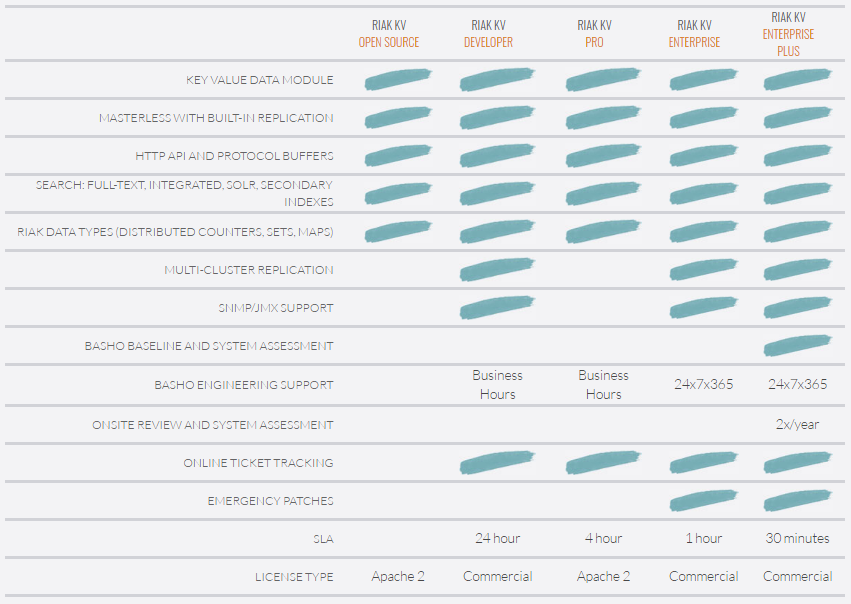
\includegraphics[width=\textwidth]{images/opensource_vs_commercial.png}
	\caption[Overview of different versions of Riak KV \protect\cite{Basho.01.04.2017}]{Overview of different versions of Riak KV \protect\cite{Basho.01.04.2017}}
	\label{fig:overview}
\end{figure}

In the following, every feature is individually viewed and explained in detail.

\newpage

\textbf{Key Value Data Module}\newline
Of course every configuration uses the key value data module developed by Basho.

\textbf{Masterless with Built-In Replication}\newline
All configurations are masterless with an integrated replication. This means that data is replicated automatically on multiple nodes so that the application remains available for both read and write operations. There is no single master and no single point of failure. This is the way the database achieves high availability. \cite{Basho.01.04.2017}

\textbf{HTTP API and Protocol Buffers}\newline
Every version works with a simple HTTP API and Protocol Buffers. Protocol Buffers is a method of serializing structured data and is especially useful for storing data. It is developed by Google. \cite{GoogleDevelopers.06.04.2017}

\textbf{Search}\newline
All implementations of the Riak KV support an integrated fulltext search and Apache Solr. Apache Solr is a popular open source enterprise search platform  built on Apache Lucene. This means with Apache Solr the user can search the whole database at once. \cite{TheApacheSoftwareFoundation.06.04.2017}

\textbf{Riak Data Types}\newline
Certainly all versions use the Riak data types which are \textit{Flags}, \textit{Registers}, \textit{Counters}, \textit{Sets} and \textit{Maps}. Flags are similar the same as Boolean, except the values are called \textit{enable} and \textit{disable}. Registers are essentially named binaries like Strings. Flags and Registers are no bucket-level Riak data types. They cannot be used on their own and have to be embedded in Maps. Counters keep track of increments or decrements. Sets are collections of unique binary values. Maps enable the creation of complex, custom data types because all other data types could be embedded. \cite{Basho.06.04.2017}

\textbf{Multi-Cluster Replication}\newline
This feature is just available for the commercial versions of Riak. The data clusters are replicated automatically in several datacenters of the customer. If one cluster fails another one provides the necessary data. \cite{Basho.01.04.2017}

\textbf{SNMP / JMX Support}\newline
SNMP means \textit{Simple Network Management Protocol} and is a protocol for collecting and organizing information about managed devices on networks. \cite{L8ManeValidus.06.04.2017} JMX stands for \textit{Java Management Extensions} and is a Java technology that provides tools for managing und monitoring applications, devices and system objects. \cite{Bryanssm.06.04.2017} Customers that use a commercial configuration of Riak are able to implement these extensions and monitor their database.

\newpage

\textbf{Basho Baseline and System Assessment}\newline
This feature is obtainable just for customers of the Enterprise Plus package. An engineer of the Basho team reviews the whole configuration of the database via remote access before Riak is deployed. \cite{Basho.01.04.2017}


\textbf{Basho Engineering Support}\newline
The Basho Engineering Support is a simple support hotline. Since the Basho team only provides payed support, this offer is not available for the open source variant. The user has to have an account to contact the support team. \cite{Basho.01.04.2017}


\textbf{Onsite Review and System Assessment}\newline
That system assessment is nearly the same as the previous one. The only difference is that the assessment is not done via remote access, but a team of engineers come to the customer’s location and review the system onsite. \cite{Basho.01.04.2017}

\textbf{Online Ticket Tracking}\newline
The Online Ticket Tracking is a functionality of the account that is needed if you do not use the open source version. In combination with the ability to contact the support team, the user can see the current state of his support ticket. \cite{Basho.01.04.2017}

\textbf{Emergency Patches}\newline
If the customers of the Enterprise versions face a problem with their database, the Basho team provides a patch as soon as possible. \cite{Basho.01.04.2017}

\textbf{Service Level Agreements}\newline
The Service Level Agreements are between 24 hours and 30 minutes response time after a problem report was sent by the customer. Afterwards the engineering team provides a solution for the problem as soon as possible. \cite{Basho.01.04.2017} 

\textbf{License Type}\newline
The last point of this comparsion is the license type. Riak KV Open Source and Riak KV Pro are available under the open source license Apache 2. The other three configurations use a commercial license. \cite{Basho.01.04.2017}

\newpage